\documentclass{article}
\usepackage{amsmath}
\usepackage{amsthm}
\usepackage{enumerate}
\usepackage[bookmarks=true]{hyperref}
\usepackage{bookmark}
\usepackage{graphicx}

\newif\ifALL

\ALLtrue

\usepackage{amssymb,amsmath,amsthm,amsfonts}
\usepackage{mathrsfs}
\usepackage{dsfont}
\usepackage{enumerate}

%\newtheorem{mdef}{Definition}
%\newtheorem{theorem}{Theorem}
\newcommand{\eqsplit}[2]{
  \begin{equation}\label{#2}
    \begin{split}
      #1
    \end{split}
  \end{equation}}
\newcommand{\eqnsplit}[1]{
  \begin{eqnarray*}
    #1
  \end{eqnarray*}}
\newcommand{\tran}[1]{
  \tilde{#1}
}
\newcommand{\td}[2]{
  \frac{d #1}{d #2}
}
\newcommand{\pd}[2]{
  \frac{\partial #1}{\partial #2}
}
\newcommand{\ppd}[2]{
  \frac{\partial^2 #1}{\partial #2^2}
}
\newcommand{\pdd}[3]{
  \frac{\partial^2 #1}{\partial #2 \partial #3}
}
\newcommand{\otd}[1]{
  \frac{d}{d #1}
}
\newcommand{\opd}[1]{
  \frac{\partial}{\partial #1}
}
\newcommand{\oppd}[1]{
  \frac{\partial^2}{\partial #1^2}
}
\newcommand{\opdd}[2]{
  \frac{\partial^2}{\partial #1 \partial #2}
}
\newcommand{\ket}[1]{
  |#1\rangle
}
\newcommand{\bra}[1]{
  \langle#1|
}
\newcommand{\inn}[1]{
  \langle#1\rangle
}
\newcommand{\mean}[1]{
  \langle#1\rangle
}
\newcommand{\tr}{
  \text{tr}\,
}
\newcommand{\re}{
  \text{Re}\,
}
\newcommand\im{
  \text{Im}\,
}
\newcommand{\var}{
  \text{var}
}
\newcommand{\arcsinh}{
  \sinh^{-1}
}
\newcommand{\arccosh}{
  \cosh^{-1}
}
\newcommand{\erfc}{
  \text{erfc}
}
\newcommand{\E}{
  \mathbb{E}
}
\renewcommand{\P}{
  \mathbb{P}
}
\newcommand{\I}[1]{
  \mathbf{1}_{\{#1\}}
}
\newcommand{\1}[1]{
  \mathds{1}_{\{#1\}}
}
\newcommand{\diag}{
  \text{diag\,}
}
\newcommand{\M}{
  {\text{max}}
}
\newcommand{\m}{
  {\text{min}}
}
\newcommand{\ph}{
  {\text{arg}\,}
}
\newcommand\erf{
  \text{erf}
}
\renewcommand\vec[1]{
  \mathbf{#1}
}
\newcommand\mtx[1]{
  \mathbf{#1}
}
\newcommand\ed{
  \,{\buildrel d \over =}\,
}



\title{On FX Rates and a Multivariate GARCH model}
\author{Xie Xiaolei}
\date{\today}
\begin{document}
\maketitle

\section{Introduction}
We study the covariance matrix of a $p$-dimensional sequence with each
component modeled by a GARCH(1, 1) process:

\begin{eqnarray*}
  X_{i,t} &=& \sigma_{i,t} Z_{i,t} \\
  (Z_{1, t}, Z_{2,t}, \dots, Z_{p,t}) &\sim& N(0, \Sigma) \\
  \sigma_{i, t}^2 &=& \alpha_{i,0} + \alpha_{i,1} X_{i, t-1}^2 + \beta_{i,1} \sigma_{i, t-1}^2
\end{eqnarray*}

\section{IGARCH(1) Processes}
We first consider the cases where $\alpha_{i, 1} + \beta_{i, 1} = 1$, i.e. IGARCH models.

\subsection{IARCH(1)}
In this case $\alpha_{i, 1} = 1$, $\beta_{i, 1} = 0$. Thus, from the equation
\begin{equation*}
  \E (Z_i^2)^{\xi_i} = 1
\end{equation*}
we obtain $\xi_i = 1$. Suppose
\begin{eqnarray*}
  \E (Z_i^2 Z_j^2)^\xi &=& 1 \\
  (Z_i, Z_j) &\sim& N(0, \Sigma) \\
  \Sigma &=&
  \begin{pmatrix}
    1 & \rho \\
    \rho & 1
  \end{pmatrix}
\end{eqnarray*}
Re-writing the above equation gives
\begin{equation}
  \label{eq:iarch1_1st}
  {1 \over 2\pi}
  \int \int
  \left(
    \rho^2 x^4 + (1 - \rho^2) x^2 y^2 + 2 \rho \sqrt{1 - \rho^2} x^3 y
  \right)^\xi
  \exp\left(
    -{x^2 + y^2 \over 2}
  \right)
  dx dy = 1
\end{equation}
When $\rho = \pm 1$, it is clear $\xi = 1/2$. When $-1 < \rho < 1$,
we may re-write \eqref{eq:iarch1_1st} in polar coordinates to obtain
\begin{equation*}
  {1 \over 2\pi} \int_0^{\infty} r^{4\xi + 1} e^{-r^2 / 2} dr
  \int_{0}^{2\pi} \cos(\theta)^{2 \xi}
  \left(
    2 \rho^2 \cos(\theta)^2
    + 2 \rho \sqrt{1 - \rho^2} \cos(\theta) \sin(\theta) - \cos(\theta)^2 + 1 - \rho^2
  \right)^\xi d\theta = 1
\end{equation*}
Integrating the radial part of the integral results in
\begin{equation*}
  \int_{0}^{2\pi}
  \cos(\theta)^{2\xi}
  \left(
    2 \rho^2 \cos(\theta)^2 + \rho \sqrt{1 - \rho^2} \sin(2\theta) - \cos(\theta)^2 - \rho^2 + 1
  \right)^\xi d\theta
  = {2 \pi
    \over
    2^{2 \xi} \Gamma(2\xi + 1)
  }
\end{equation*}
After some manipulations we arrive at
\begin{equation}
  \label{eq:iarch_2nd}
  \int_{-1}^1 (\sin(\pi z) + \rho)^{2\xi} dz = {2 \over \Gamma(2\xi + 1)}
\end{equation}
Using this result, we immediately obtain for ARCH(1) models
\begin{equation*}
  \label{eq:arch_1st}
  \int_{-1}^1 (\sin(\pi z) + \rho)^{2\xi} dz =
  {2 \over \Gamma(2\xi + 1)}
  {1 \over (\alpha_{i, 1} \alpha_{j, 1})^\xi}
\end{equation*}
Fitting ARCH(1) models to the FX return series and then simulating the
models produces a fairly good match between the spectra of the
simulated and the real series, as shown in figure
\ref{fig:FX_ARCH_eigenvalues} and \ref{fig:FX_ARCH_eigenvectors}.
\begin{figure}[htb!]
  \centering
  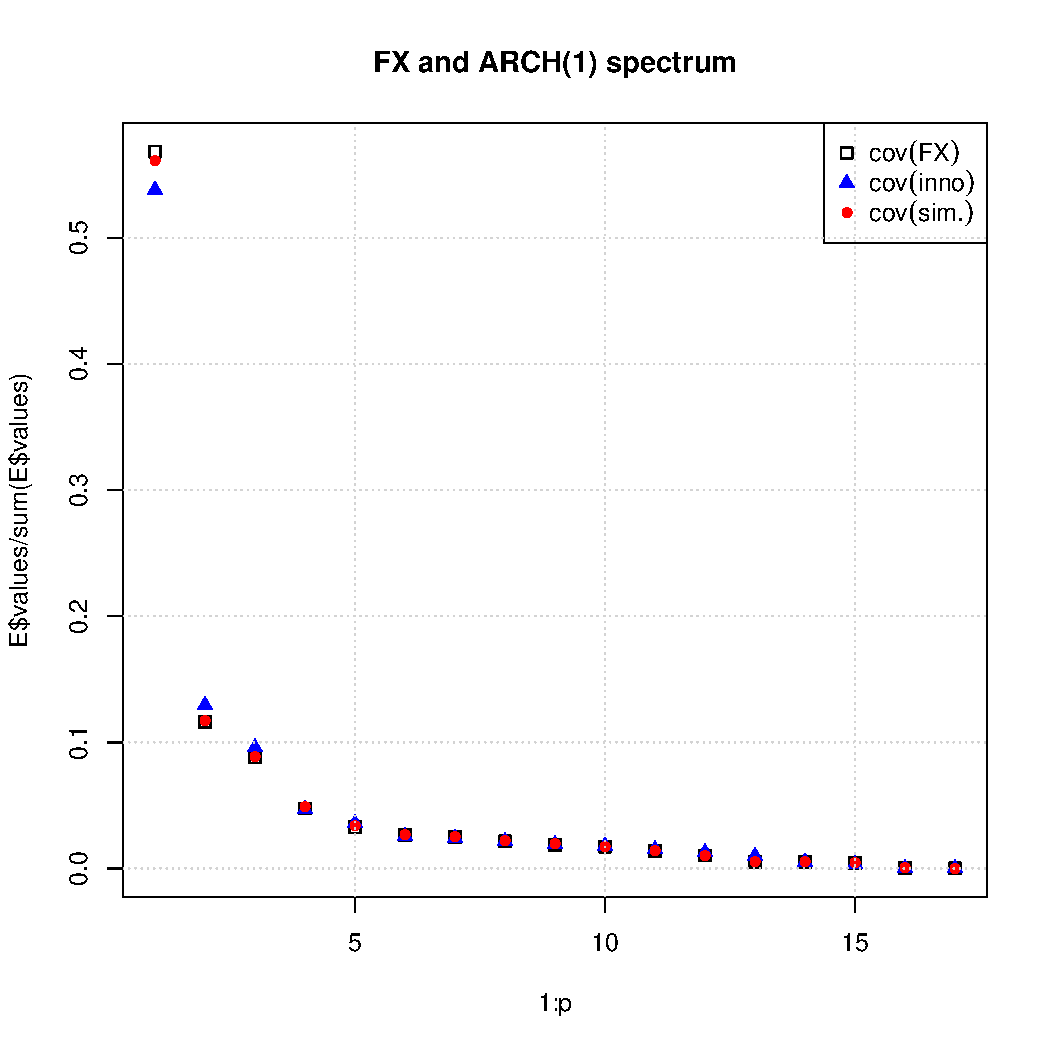
\includegraphics[scale=0.4]{FX_eigenvalues.pdf}  
  \caption{FX \& simulated ARCH eigenvalues}
  \label{fig:FX_ARCH_eigenvalues}
\end{figure}

\begin{figure}[htb!]
  \centering
  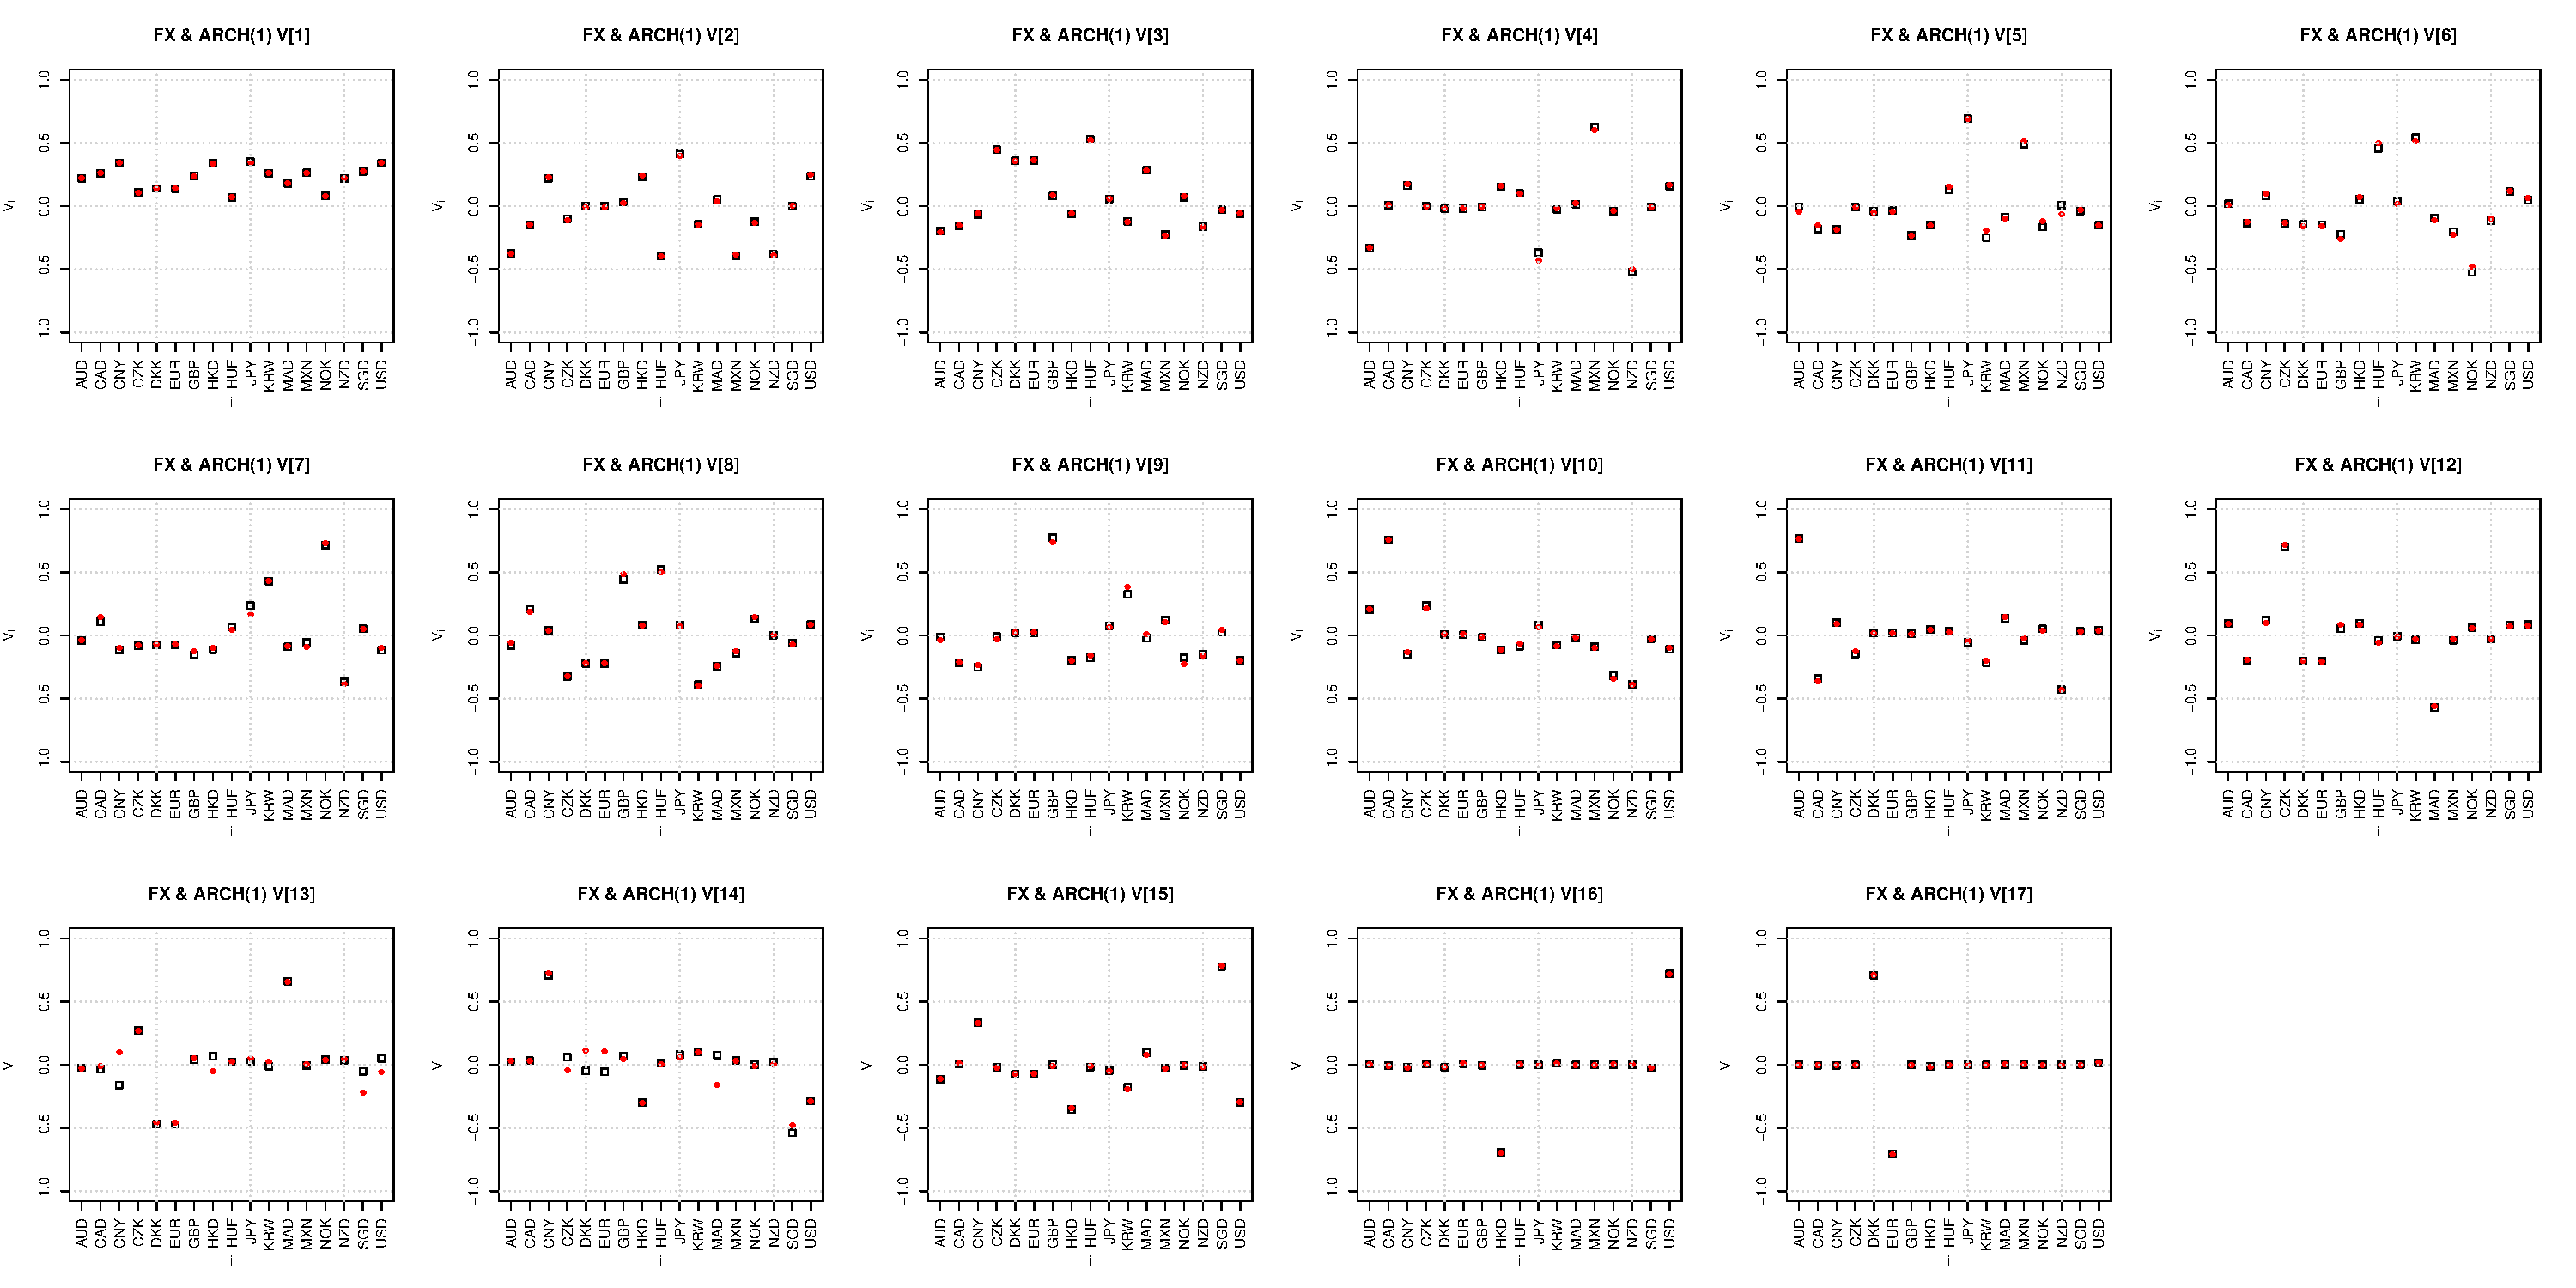
\includegraphics[scale=0.3]{FX_eigenvectors.pdf}  
  \caption{FX \& ARCH eigenvectors}
  \label{fig:FX_ARCH_eigenvectors}
\end{figure}

\section{General IGARCH(1)}
For general IGARCH(1) models, the equation
\begin{equation*}
  \E \left[
    (
    \alpha_{i,1} Z_1^2 + 1 - \alpha_{i,1}
    )^\xi
    (
    \alpha_{j,1} Z_2^2 + 1 - \alpha_{j,1}
    )^\xi\right] = 1
\end{equation*}
has to be solved numerically. Figure \ref{fig:xi_rho0.5} shows $\xi$
as a function of $(\alpha_{i,1}, \alpha_{j,1})$ as defined by the
above equation.
\begin{figure}[htb!]
  \centering
  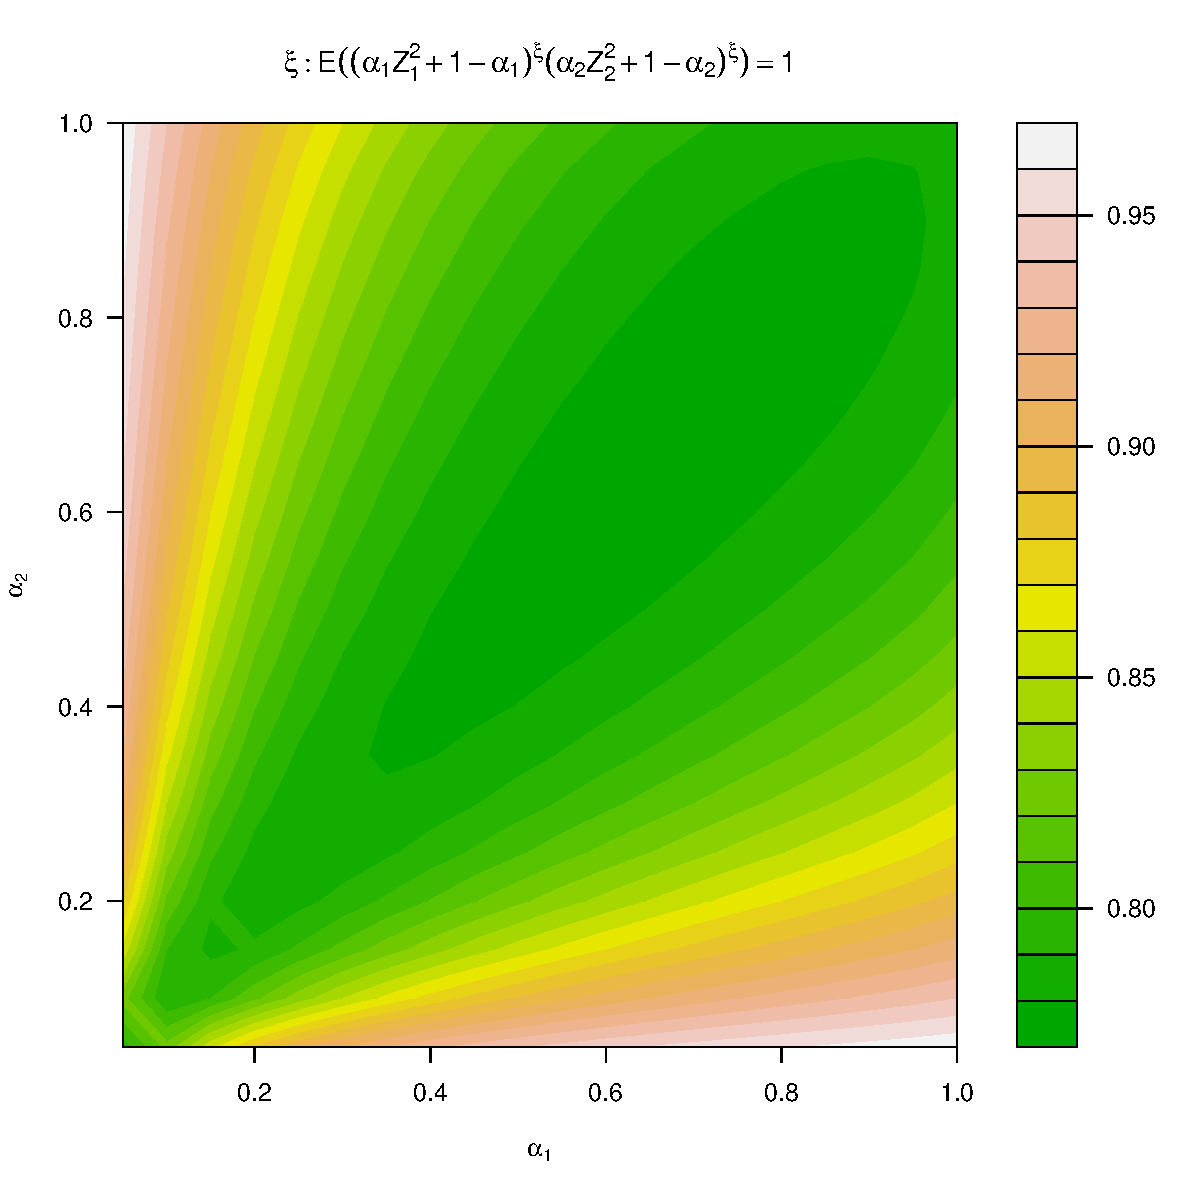
\includegraphics[scale=0.4]{igarch_rho0dot5.pdf}
  \caption{$\xi(\alpha_1, \alpha_2)$ for $\rho = 1/2$}
  \label{fig:xi_rho0.5}
\end{figure}

\section{Heavy-Tailed Innovations}
Figure \ref{fig:ARCH_t_FX_eigenvalues} and Figure
\ref{fig:ARCH_t_FX_eigenvectors} show the eigenvalues and
eigenvectors of the simulated GARCH(1, 1) process with innovations
following t(4) distribution. Clearly, the spectrum of the simulated
series does not match that of the observed FX series.
\begin{figure}[htb!]
  \centering
  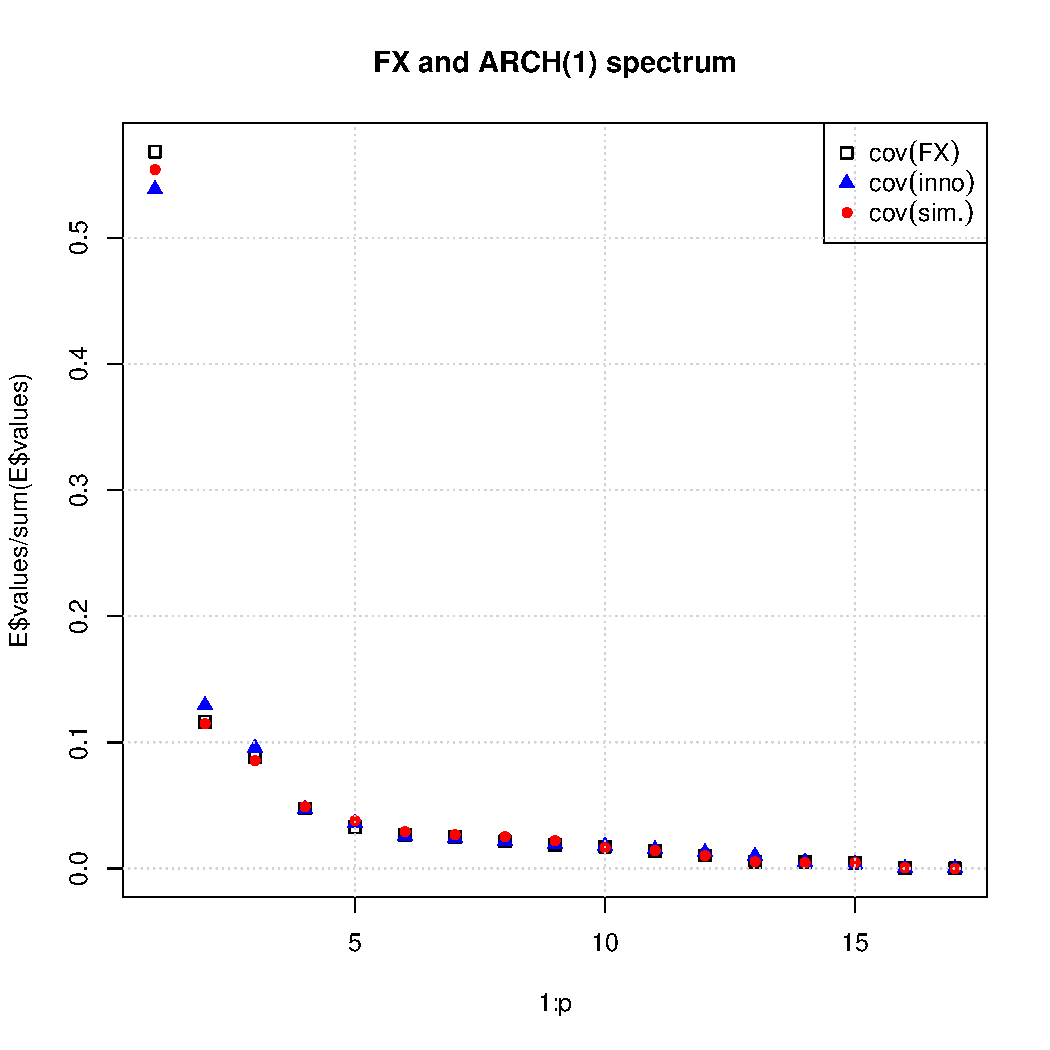
\includegraphics[scale=0.4]{FX_eigenvalues_ARCH_t_inno.pdf}  
  \caption{FX \& simulated ARCH eigenvalues. t-distributed innovations}
  \label{fig:ARCH_t_FX_eigenvalues}
\end{figure}

\begin{figure}[htb!]
  \centering
  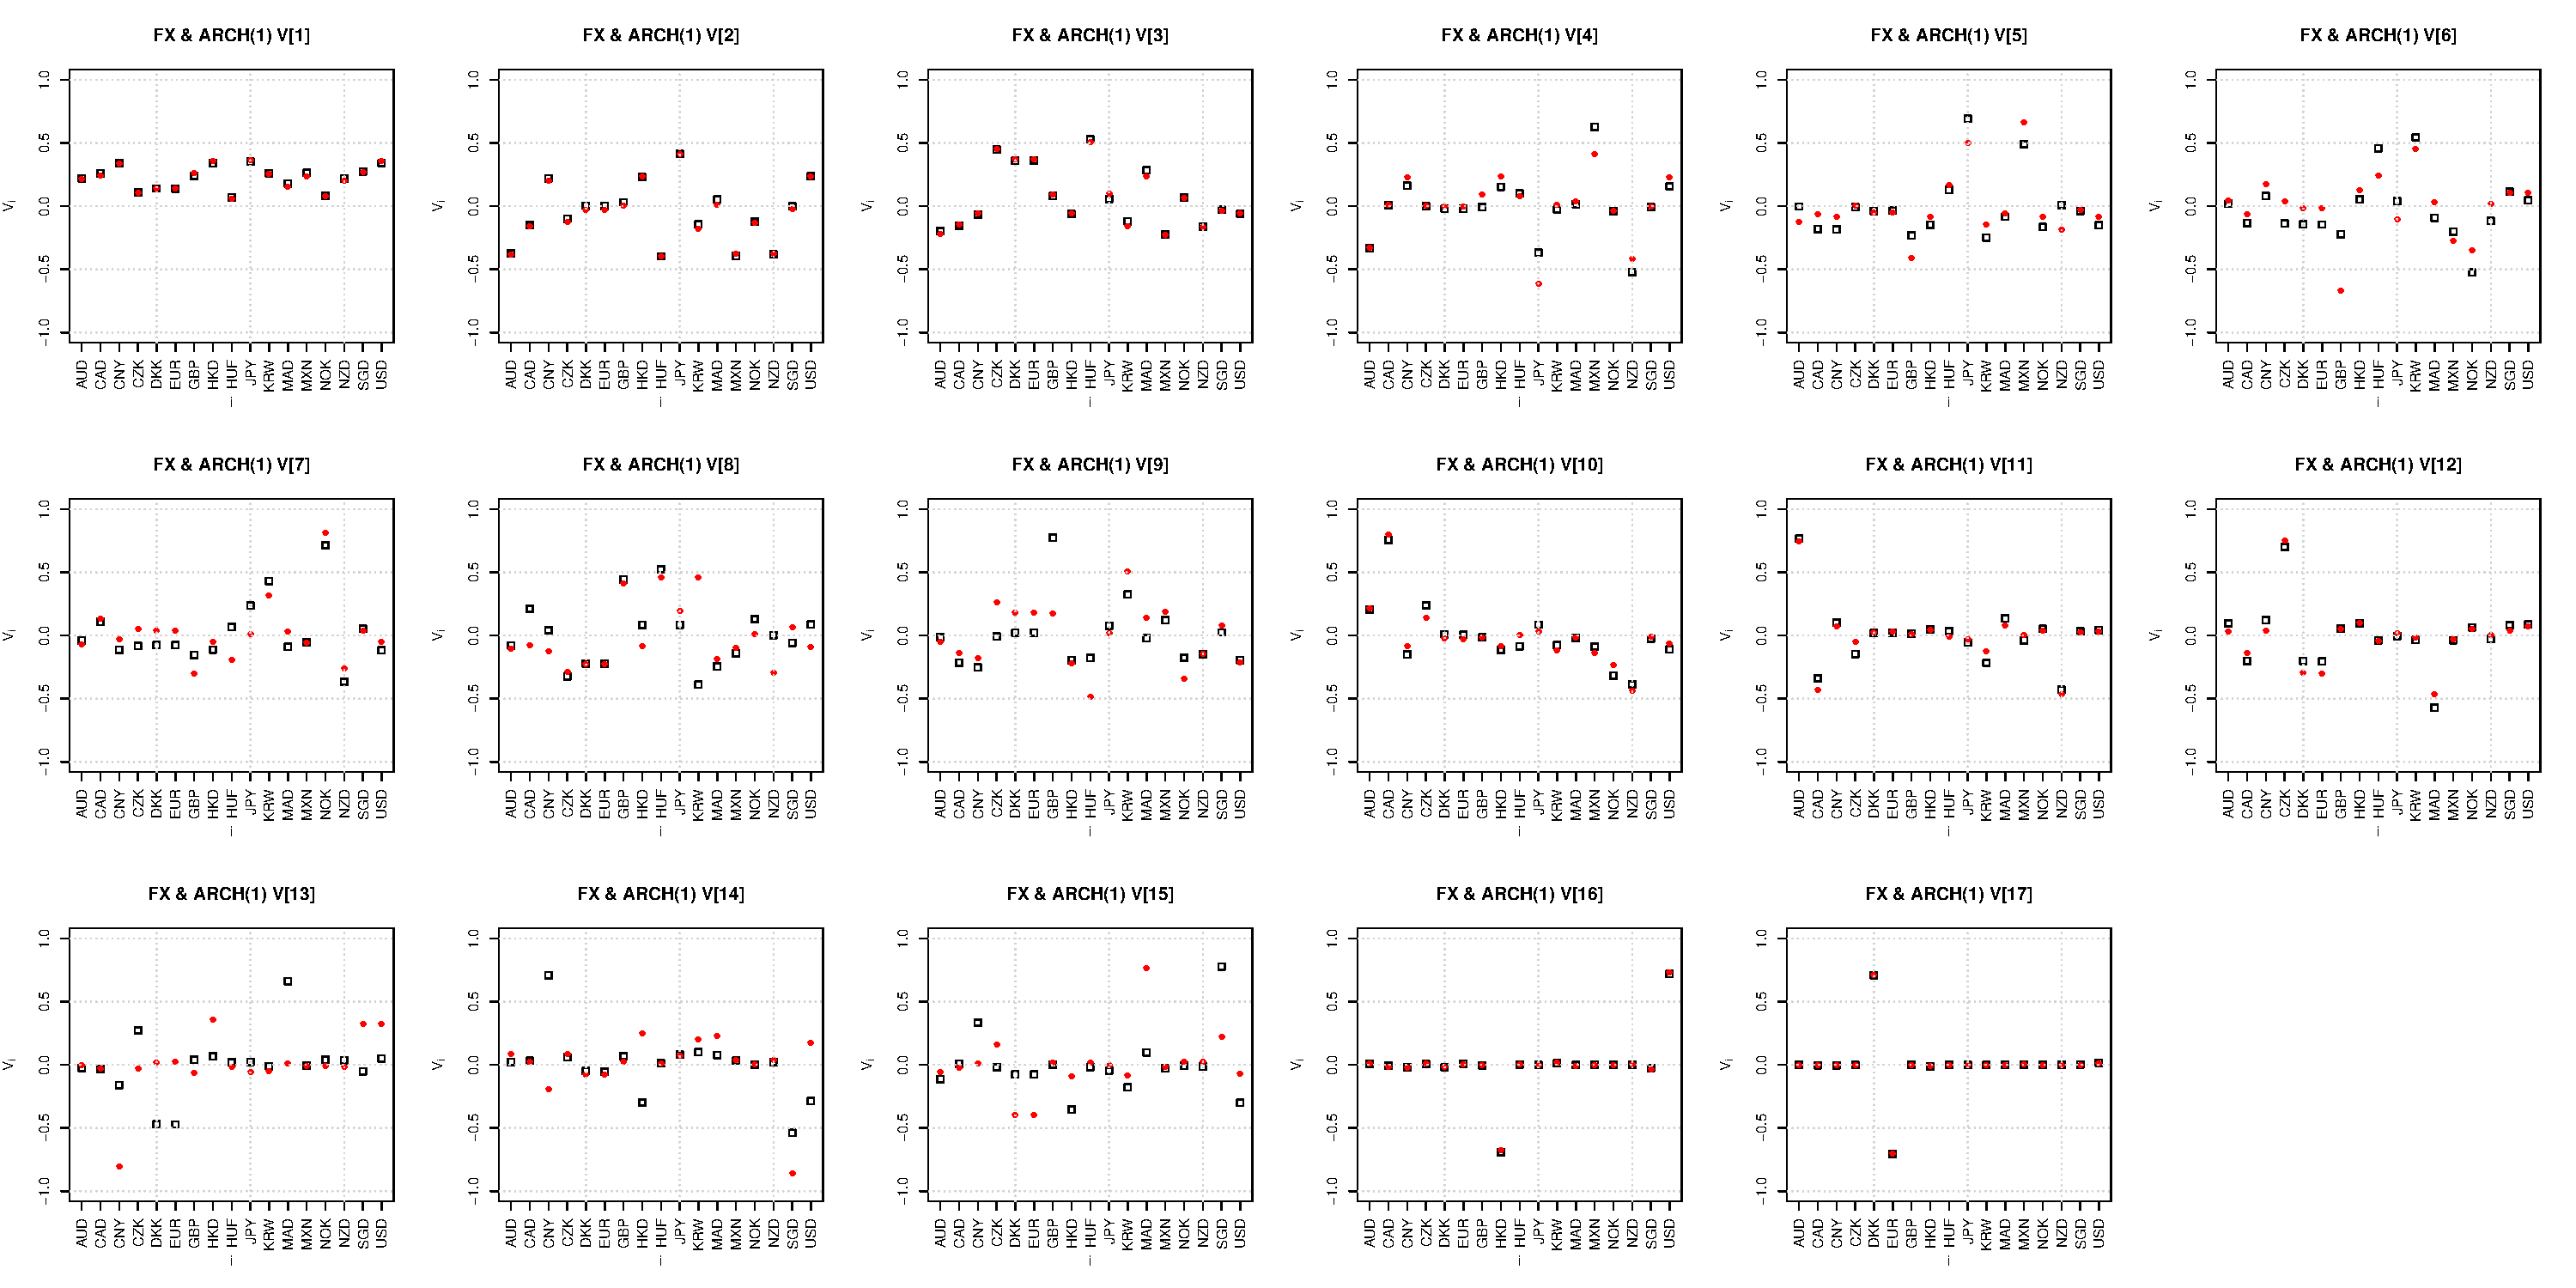
\includegraphics[scale=0.3]{FX_eigenvectors_ARCH_t_inno.pdf}  
  \caption{FX \& ARCH eigenvectors. t-distributed innovations}
  \label{fig:ARCH_t_FX_eigenvectors}
\end{figure}


\section{Spectra of S\&P sectors}
\subsection{Utilities}
Fitting the daily returns' data of 25 companies that have been
included in the S\&P 500 index since 2010-01-01 and categorized in the
sector ``Utilities'', we obtained 23 GARCH(1, 1) models that satisfy
the condition
\begin{equation}
  \label{eq:garch_cond1}
  \alpha_1 + \beta_1 < 1  
\end{equation}
Then we simulate the GARCH(1, 1) processes with innovations having the
same covariance structure as those of the real data. Figure
\ref{fig:Utilities_eigenvalues} and \ref{fig:Utilities_eigenvectors1},
\ref{fig:Utilities_eigenvectors2}
compare the eigenvalues and eigenvectors, respectively, of the 
covariance matrices of the real and the simulated data.
\begin{figure}[htb!]
  \centering
  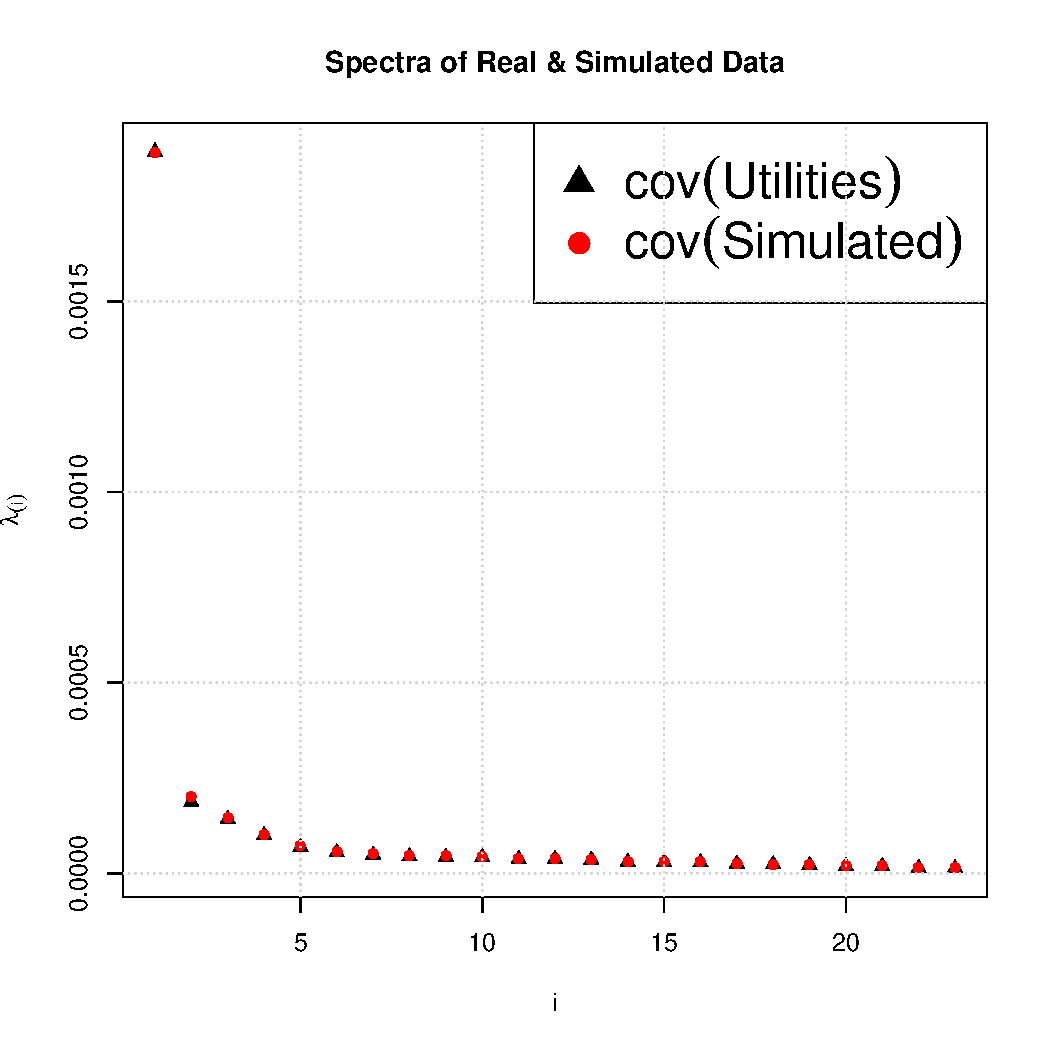
\includegraphics[scale=0.4]{Utilities_eigenvalues.pdf}
  \caption{Eigenvalues of Utilities: real \& simulated}
  \label{fig:Utilities_eigenvalues}
\end{figure}

\begin{figure}[htb!]
  \centering
  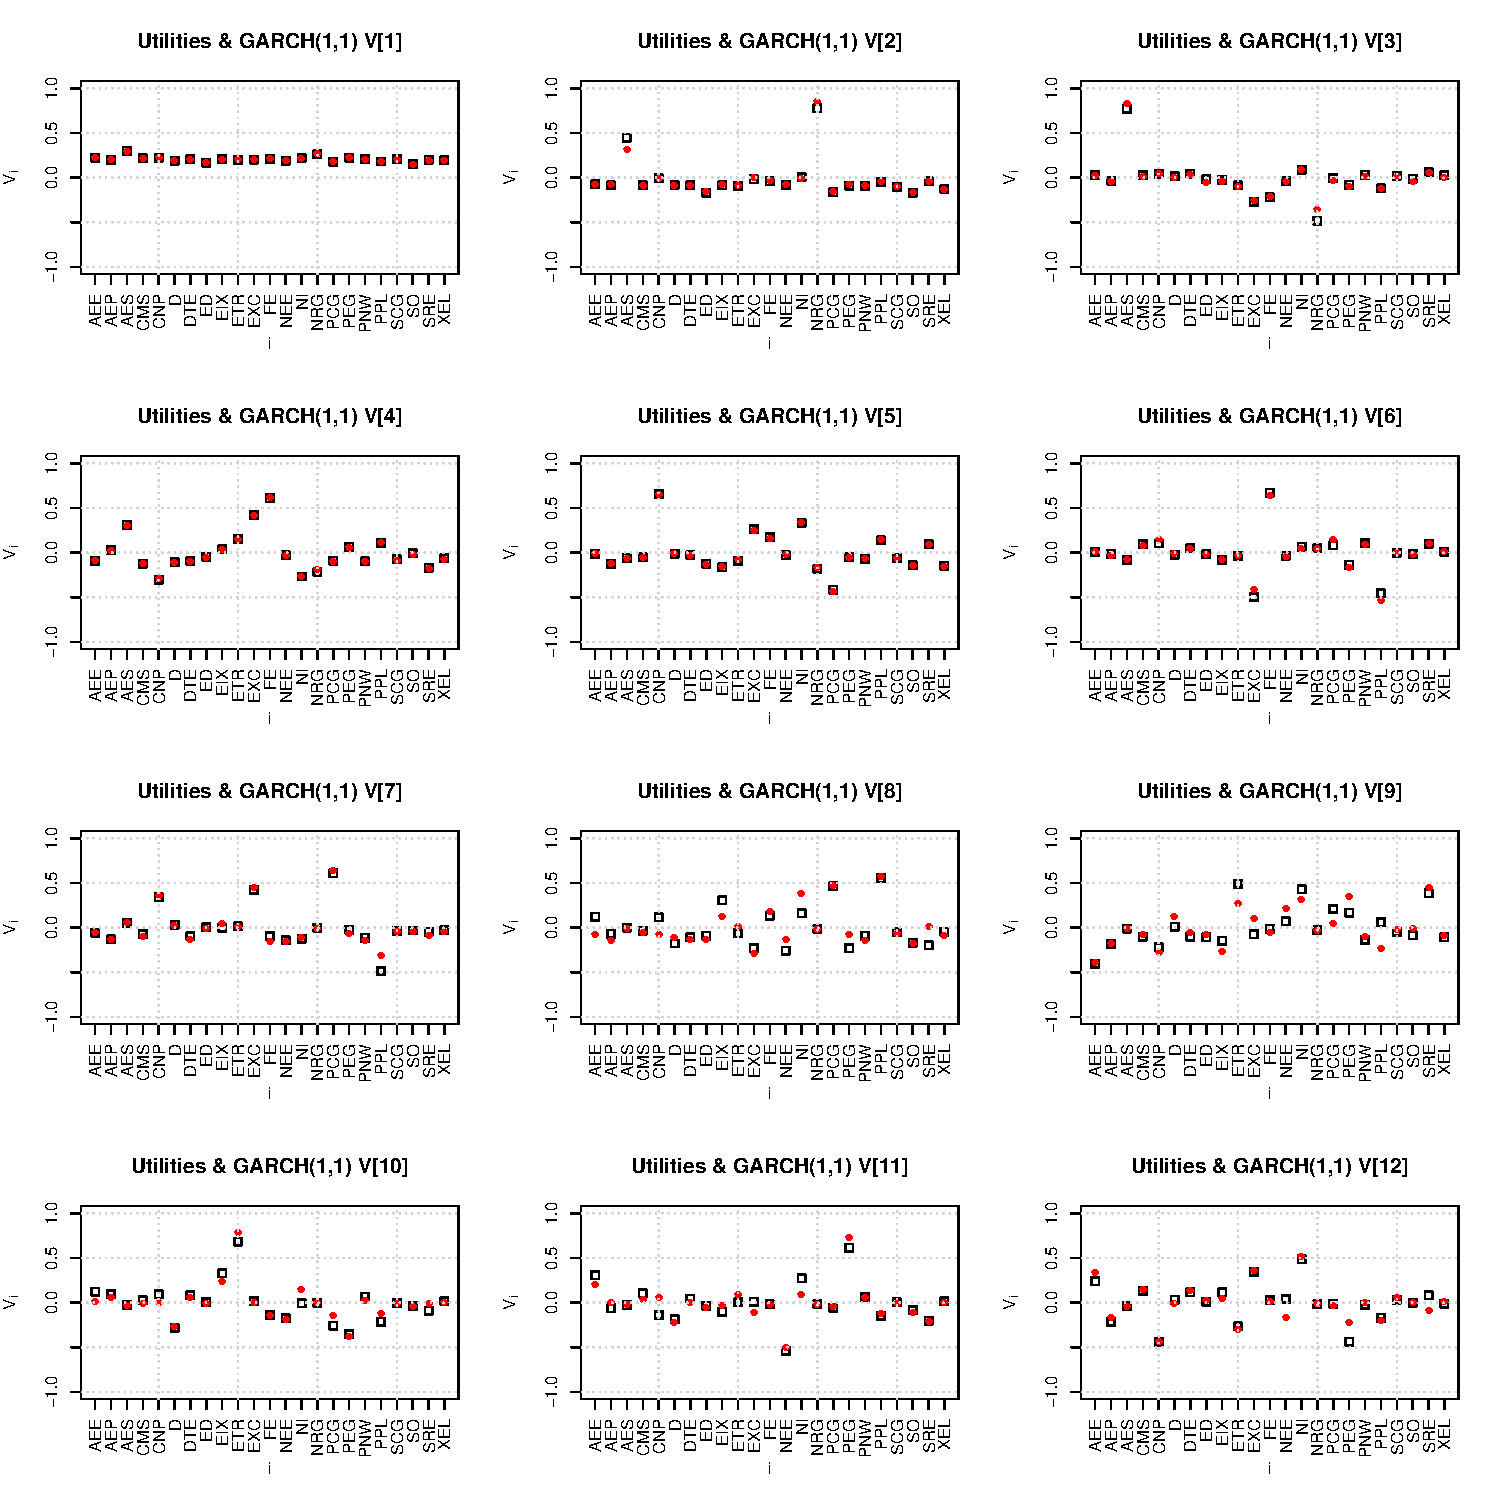
\includegraphics[scale=0.5]{Utilities_eigenvectors1.pdf}
  \caption{Eigenvectors of Utilities: real \& simulated}
  \label{fig:Utilities_eigenvectors1}
\end{figure}

\begin{figure}[htb!]
  \centering
  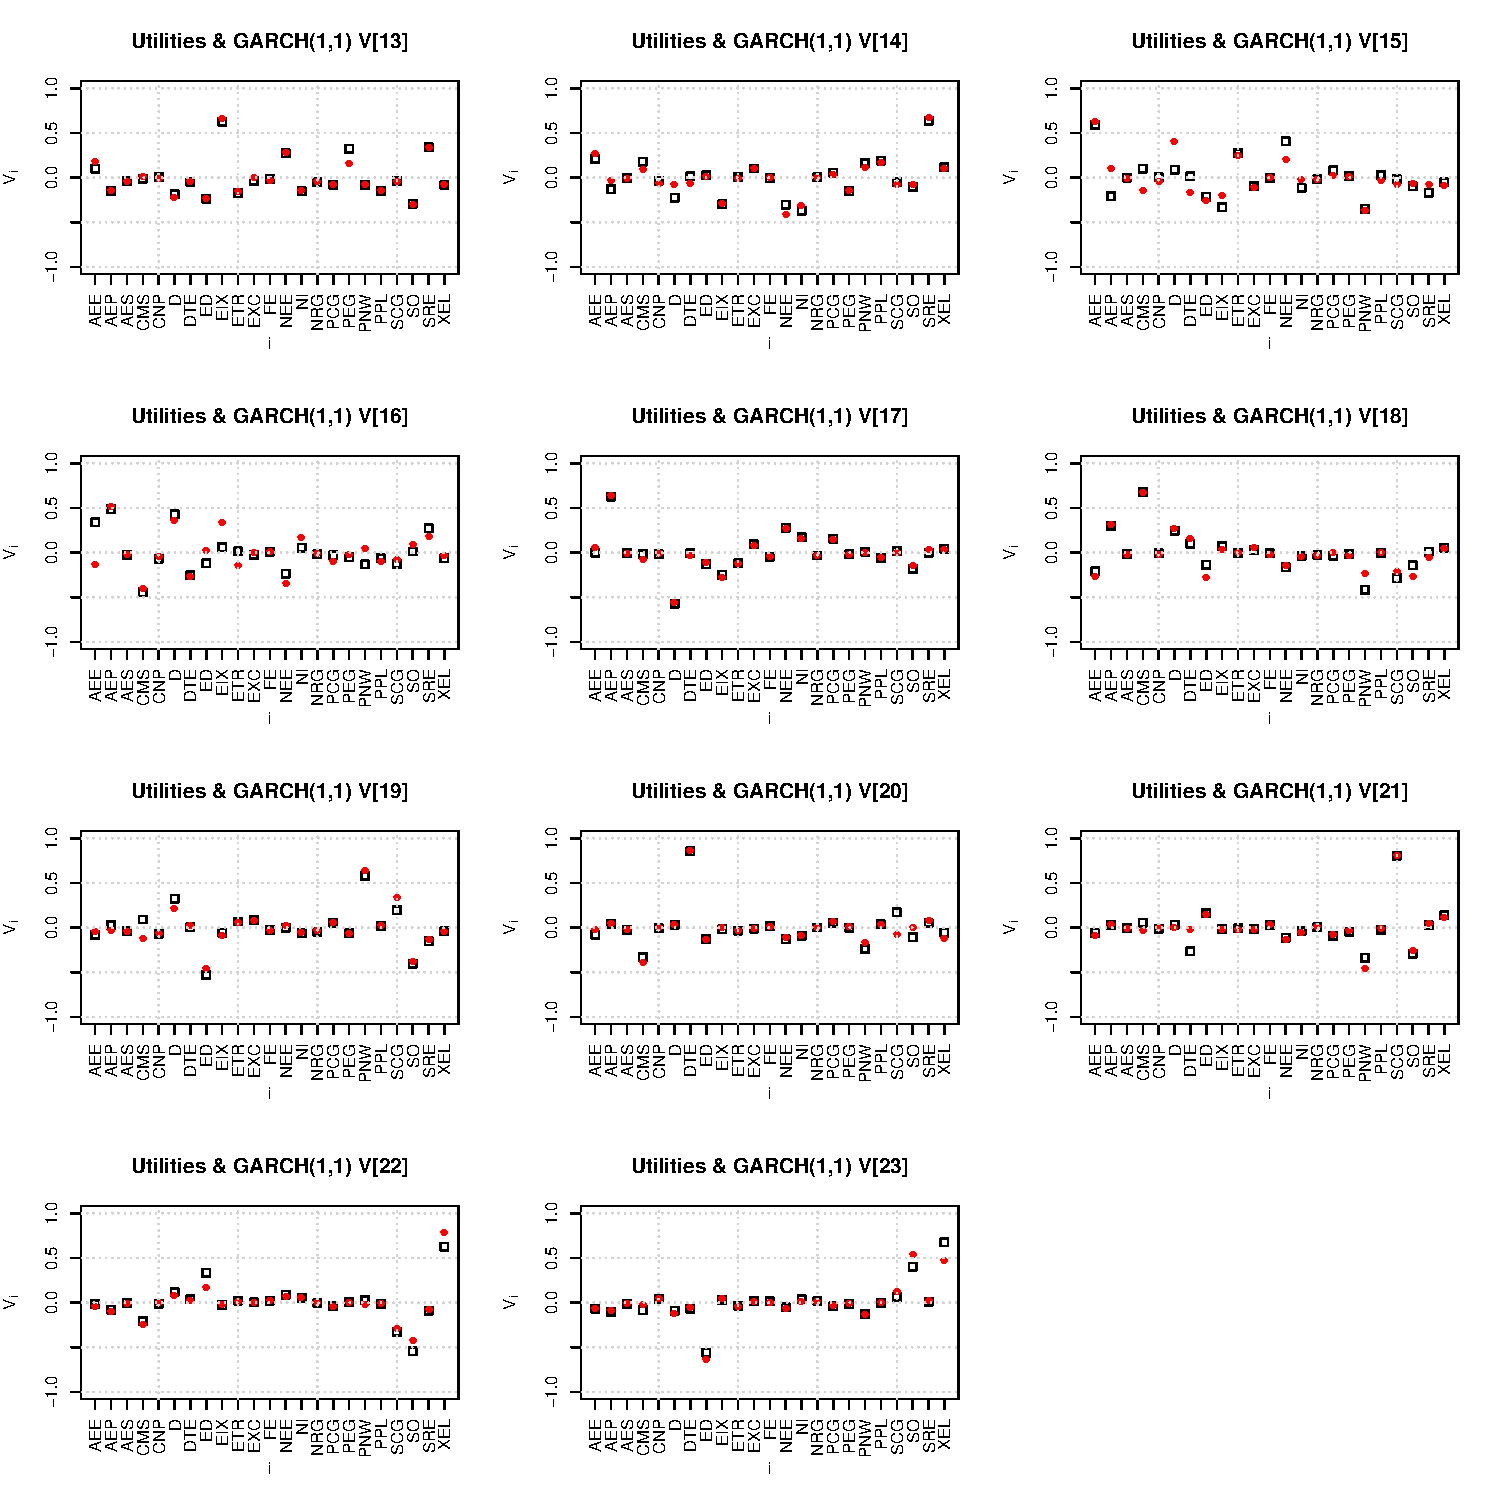
\includegraphics[scale=0.5]{Utilities_eigenvectors2.pdf}
  \caption{Eigenvectors of Utilities: real \& simulated continued}
  \label{fig:Utilities_eigenvectors2}
\end{figure}

\subsection{Materials}
A similar analysis on the ``Materials'' sector produces the following
spectra. In this sector, 21 out of 25 return sequencies are
successfully fitted to GARCH(1, 1) models that satisfy condition
\eqref{eq:garch_cond1}.

\begin{figure}[htb!]
  \centering
  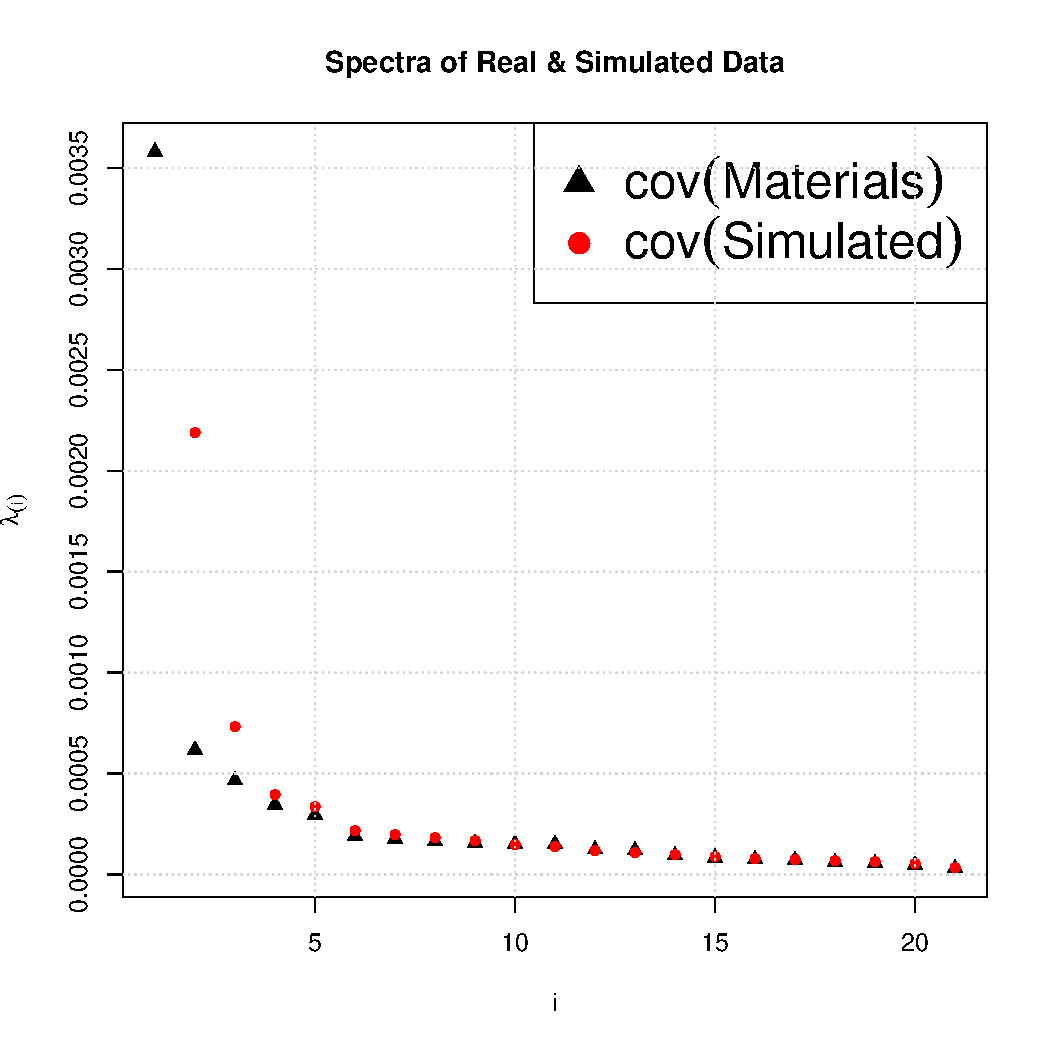
\includegraphics[scale=0.6]{Materials_eigenvalues.pdf}
  \caption{Eigenvalues of Materials: real \& simulated}
  \label{fig:Materials_eigenvalues}
\end{figure}

\begin{figure}[htb!]
  \centering
  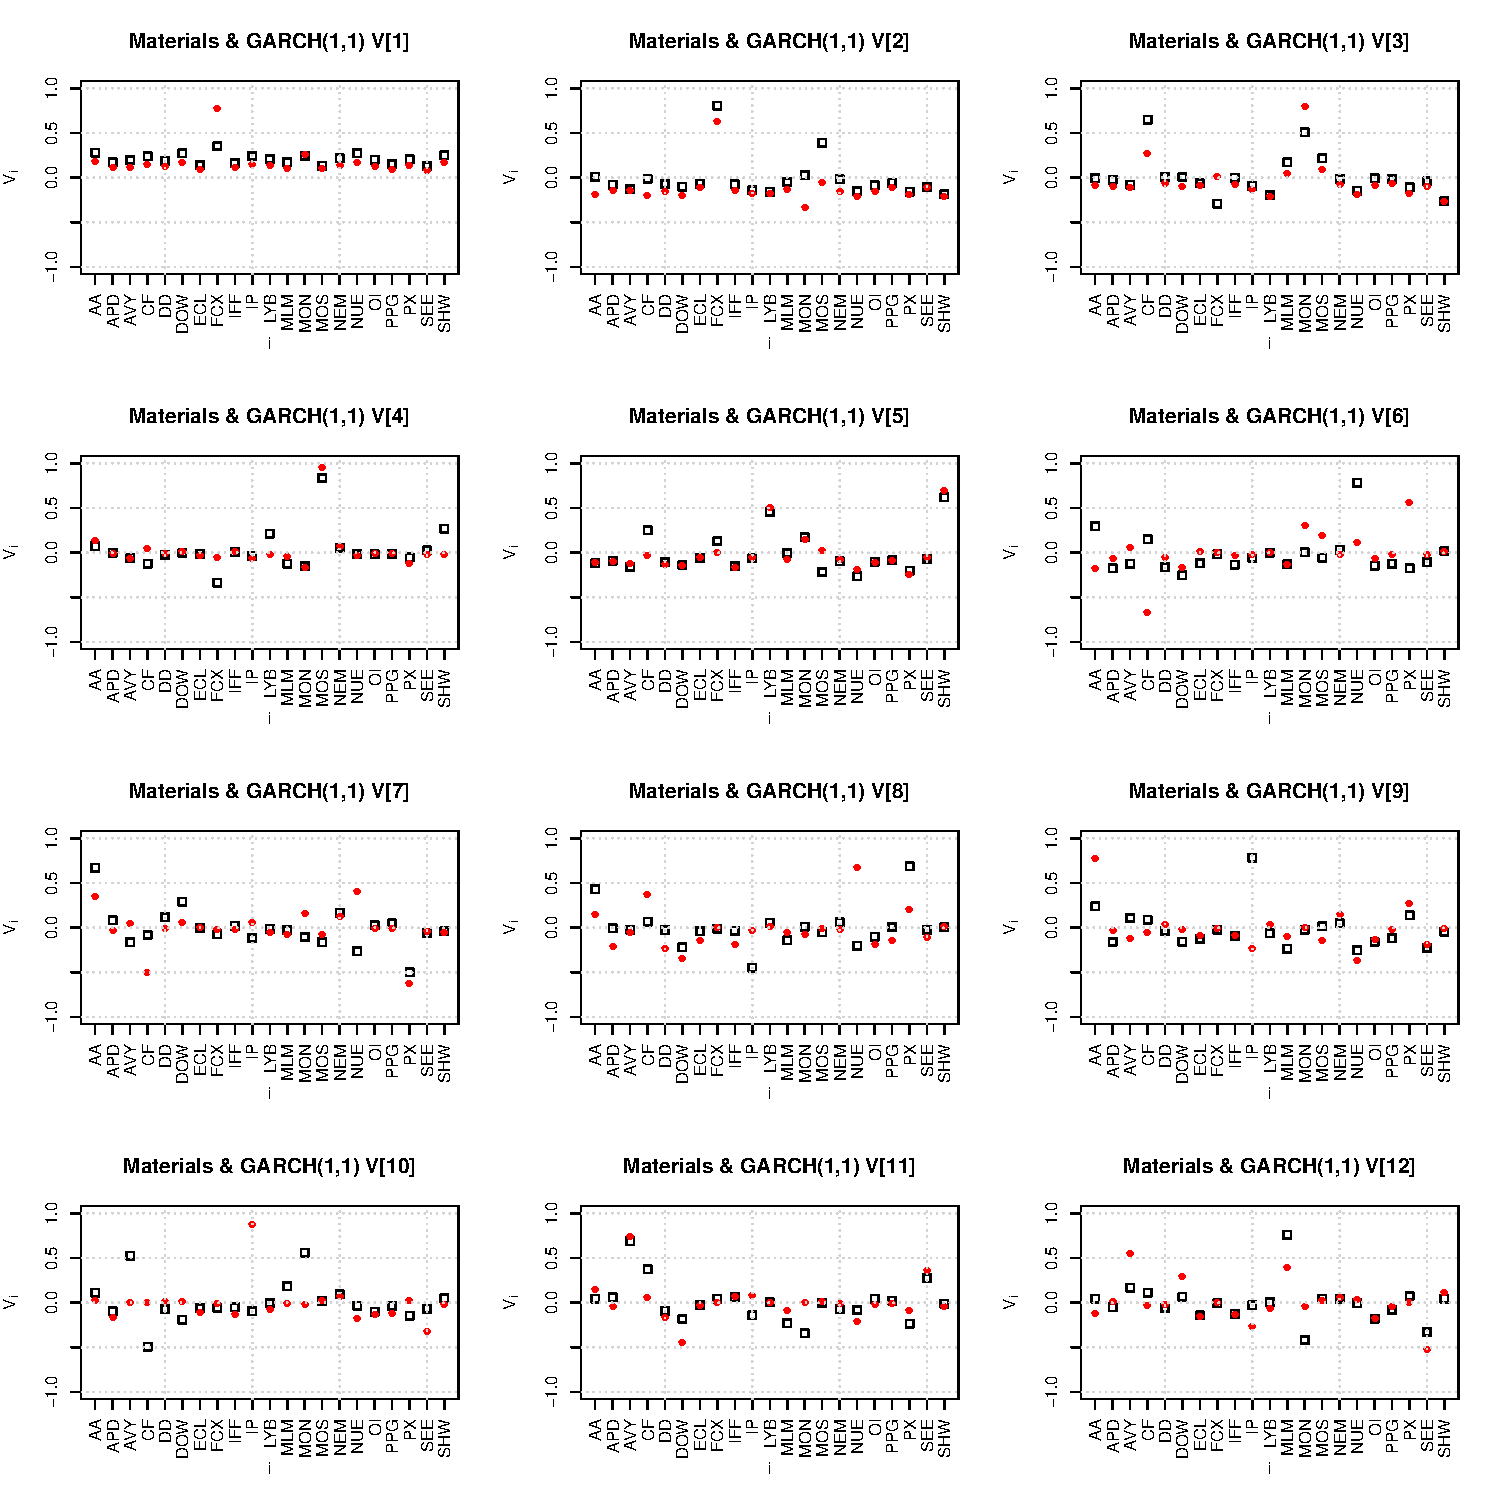
\includegraphics[scale=0.5]{Materials_eigenvectors1.pdf}
  \caption{Eigenvectors of Materials: real \& simulated}
  \label{fig:Materials_eigenvectors1}
\end{figure}

\begin{figure}[htb!]
  \centering
  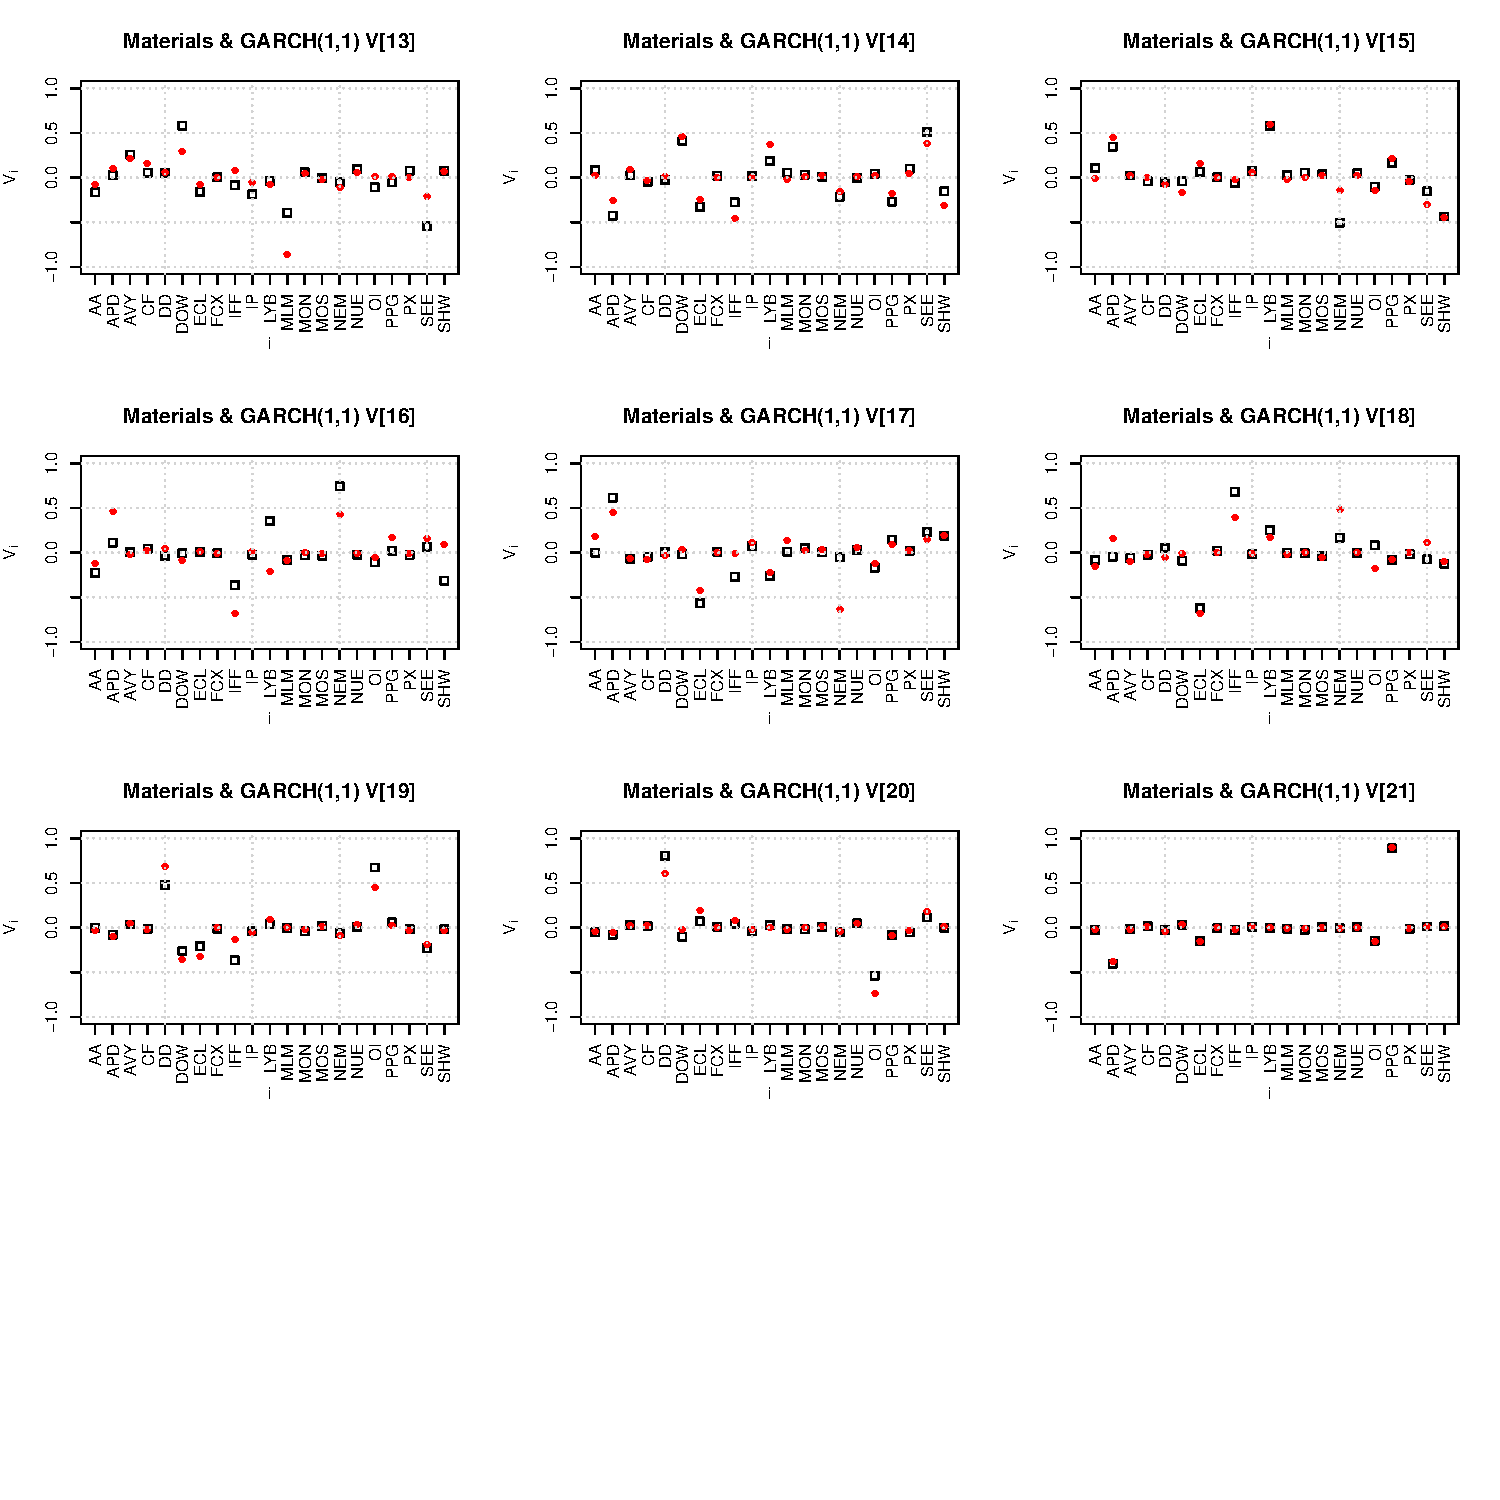
\includegraphics[scale=0.5]{Materials_eigenvectors2.pdf}
  \caption{Eigenvectors of Materials: real \& simulated continued}
  \label{fig:Materials_eigenvectors2}
\end{figure}

\bibliographystyle{unsrt}
\bibliography{../thesis/econophysics}
\end{document}
